\section{Google}
\label{secc:google}

Un punto importante en lo que al desarrollo de aplicaciones móviles se refiere, es el uso que los usuarios dan a las aplicaciones, hay muchas aplicaciones en el mercado de la tecnología móvil, pero las aplicaciones punteras que salen adelante son las que tiene compatibilidad con otras aplicaciones que usan habitualmente los usuarios como puede ser el correo, las redes sociales, o sin necesidad de ese tipo de funcionalidades, las usan porque son realmente originales en su ámbito.
Google ha hecho un negocio de las aplicaciones y facilita a los desarrolladores a que  realicen aplicaciones proporcionando APIs de sus productos y permitiendo que suban las aplicaciones a su tienda.
En este apartado se detallará el uso de Google dentro de aplicaciones del tipo de aplicación que es Baldugenda, una aplicación que controla calendarios, realiza backups de información  y tiene control de cuentas de Google.

\subsection{Google Play}
\label{subsecc:Google Play}

Para empezar Google proporciona la posibilidad de compartir  las aplicaciones por medio de Google Play.

Para poder desarrollar aplicaciones y colgarlas en el Play Store hay que realizar un pago de 25\$, con ese pago se consigue que la cuenta de Gmail escogida pase a ser de desarrollador, lo que permite crear aplicaciones y subirlas, también se puede monetizar esas aplicaciones por medio de publicidad.

Una vez se ha realizado el pago la creación de una aplicación se separa en dos partes principales.

\begin{itemize}
\item Desarrollo mediante Eclipse o \gls{Android Studio}
\item Subida al Google Play
\end{itemize}

Para programar en Android la mejor opción es la de Android Studio, ya que genera los ficheros y el manifest del proyecto sin tener que estar modificándolo todo el rato.
Si se escoge la opción de Eclipse ya Google no da el soporte necesario y es más complicado programar en él.
Dentro de Android Studio hay varias posibilidades a la hora de crear un proyecto y depende de cuál se escoja funcionara para distintos dispositivos.
Cuando se ha creado el proyecto y se ha conseguido probar sin errores hay que firmar el apk, para esto Android Studio permite generar un apk firmada de una manera fácil.

\newpage
\begin{figure}[H] 
  \begin{center} 
    \scalebox{1}{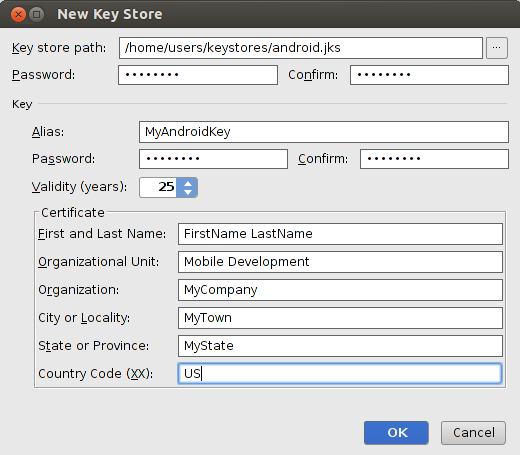
\includegraphics{figs/CreacionKey.png}} 
    \caption{Ventana de creación de Key} 
    \label{fig:CreaciónKey} 
  \end{center} 
\end{figure}

Con la ventana anterior se genera un fichero que se usará como llave para firmar la aplicación, en el caso de necesitar usar APIs de google se necesitará de la contraseña cifrada en Sha1 para enlazar el API con la aplicación.


La parte más pesada después de desarrollar la aplicación es el papeleo con Google, para subir cualquier aplicación hay que rellenar muchos campos dentro del formulario para que Google permita subir la aplicación. Estos campos la mayoría son información de la aplicación como imágenes del icono que usaremos, el tipo de aplicación que es, qué tipo de gente puede usarla, y otras preguntas parecidas a las anteriores.

Una vez Google permita colgar la apk, dará 3 opciones,  en producción, beta  o alfa. Estas opciones limitaran la cantidad de gente que se puede descargar la aplicación. Y ayuda a tener una versión de la aplicación funcionando mientras se está probando una versión superior en otro tipo de subida.
Si se quiere compartir en alpha o en beta hay 2 opciones para agregar a mucha gente a la vez, la primera opción es la que se usó durante la primera fase de las pruebas con los Baldusers, que es creando una comunidad de Google plus y dentro poniéndoles el link para que se la descargasen. O la segunda opción que se usó en la segunda fase de las pruebas, que se creó un grupo de Google groups y se añadió los emails de la gente y dentro de la invitación se les añadió el link de descarga, se limitó los permisos de la gente del grupo para que no pudieran crear nada ni responder a nadie.

La primera opción dio muchos fallos ya que había gente que por el tipo de cuenta que usaban en su universidad o instituto no se les permitía usar Google plus así que no podían asociarse al grupo de usuarios por esa forma, aparte si no se tenía cuenta en Google plus, esta opción les obligaba a crearse cuenta con el coste de tener que explicarles paso a paso como hacerlo si no eran muy entendidos de las redes sociales.
La segunda opción y en mi opinión la más útil fue la de crear los grupos mediante Google Groups, el Balduser solo recibía un email con 2 links, uno para aceptar la invitación y otro para unirse a las pruebas de la descarga de la aplicación. No tenían que hacer nada más. Lo bueno de esta opción es que se estaba trabajando con el grupo de Baldusers como si fuera una lista de emails y en el caso de tener que mandar una información general solo había que redactar un correo de grupo.

Una vez seleccionado los grupos que tenían acceso a la aplicación en fase alpha el siguiente paso era subir la apk.
La subida a Google play no es inmediata, por esta razón cuando se subía Baldugenda solían pasar un par de horas hasta que la descarga estuviera disponible.
Unos puntos importantes a la hora de generar las aplicaciones son el peso de la aplicación, los dispositivos a los que va dirigido y los permisos que se pedirán a los usuarios.
Los dos primeros puntos están vinculados, ya que si se escoge un grupo muy amplio de dispositivos tanto por pantalla como por versión de Android, se estará ante una situación en la que para que se vea correctamente en todos los dispositivos habrá que meter iconos de diferentes tamaños y generar vistas dependiendo del dispositivo.

Siempre hay que pensar que no es lo mismo desarrollar una aplicación web que una aplicación móvil, los dispositivos móviles no disponen de mucha capacidad de almacenamiento así que cuanto menos pese la aplicación, más posibilidades hay de que no de problemas para a la hora de instalarla.
Aparte de los iconos y las vistas también dependemos de las librerías cuanto más alta es la versión de Android más peso añade al programa a la hora de la instalación porque le añade funciones nueva de las librerías aunque no las hayamos usado, como puede ser un cambio de color al pulsar un botón, que aunque en nuestro código no se pueda ver, ni en las versiones anteriores se vea, cuanto mayor es la API más funciones agrega.
Google limita el peso de las apk que se pueden subir a Google Play en 50 mb, a partir de ese peso se pueden subir extensiones para la aplicación.

\subsection{Uso de APIs}
\label{subsecc:Uso de APIs}

Ya se ha explicado cómo funciona la subida de una aplicación a Google play, pero eso no es lo único que Google proporciona de ayuda a la hora de desarrollar la aplicación y distribuirla.
Google proporciona sus APIs propias para que se vinculen los servicios que ofrece Google con la aplicación que se quiera desarrollar. Si la aplicación que se quiere desarrollar no va a realizar un gran uso de los servicios de Google no hay problema, el problema surge cuando se alcanza el límite de usos de la API y Google exige pagos para seguir usándolo al mismo rendimiento.
Aunque a priori las cuotas parecen altas siendo como es el caso de Google Calendar API \cite{GCalendar} de 1.000.000 de solicitudes por día, si una aplicación se quisiera comercializar ya habría que estar al tanto de cuantas solicitudes se realizan y si se necesita aumentar la cuota, puesto que al tener publica la aplicación, cualquiera en el mundo podria descargarsela.

Para el uso de estas APIs, Google ofrece distintas posibilidades dependiendo de la API, ya que hay algunas que necesitan autenticación para funcionar como puede ser el caso de Google Calendar frente a otras como Google maps que lo único que necesitan es la credencial de tu aplicación para llevar al día la cuota de la API.
Este apartado de credenciales de las APIs es un tema bastante difícil a la hora de usar los servicios de Google y donde más problemas se suelen tener. Google lo explica en su web paso a paso como configurar las credenciales. Aunque bastantes veces habrá que generar credenciales que no se sabe para qué sirven porque las que dice Google que se generen no dan acceso a la API.

Dentro de la consola de desarrollador de Google es donde hay que añadir los certificados del API, hay distintas pestañas, algunas dan información del uso que se ha dado del servicio y otras dan la posibilidad de agregar más servicios al proyecto.
Se pueden encontrar servicios tales como el Google Calendar o el Drive que se han usado para la parte de la administración de calendarios y el backup dentro de Baldugenda, como también podemos encontrar servicios de youtube, traductor, publicidad, mapas. 

Todos los productos que Google quiere vender al alcance de los desarrolladores.
Lo bueno que tiene usar los servicios de Google es que todo aquel que se descargue la aplicación habrá usado alguna vez esos servicios o tenga la aplicación instalada en su dispositivo aunque no la use. Si se usaran servicios de terceros que no fuera Google se tendría que pedir al usuario que se creara otra cuenta o que se instalara otra aplicación para poder sacar todo el partido a la aplicación que se está creando.

La finalidad de usar servicios de terceros de empresas importantes en los dispositivos móviles es, que los usuarios usen el producto que se ha desarrollado y que no se lo desinstalen, uno de los motivos por los que la gente desinstala aplicaciones pequeñas es que les exigen estar duplicando información que quieren tener centralizada. Un ejemplo podría ser los eventos del calendario, hay muchas aplicaciones que usan el calendario del móvil pero que no dan soporte a calendarios online como el de Google Calendar, en este caso si el usuario quiere crear un evento con esa aplicación no puede modificarlo desde el ordenador y le limita a usar siempre el móvil con ese evento.
Pasa lo mismo con las notas o con los ficheros al querer guardarlos en los móviles, generando así una necesidad para el usuario de tener un espacio de almacenamiento enorme si quiere sacar fotos y descargase cualquier cosa al móvil.

\subsection{Uso de calendarios}
\label{subsecc:Uso de calendarios}

En el apartado anterior se ha hablado de las APIs,  una de las que proporciona Google es la de Google Calendar, en las aplicaciones parecidas a Baldugenda el uso de Google Calendar no es habitual la mayoría generan los horarios en calendarios propios de la aplicación y te muestran fechas del calendario solo accesibles desde el móvil.
Google al proporcionar el API de Google Calendar y al estar tan vinculado a Android para descargar las aplicaciones proporciona una relación con el calendario del móvil casi perfecta tanto para visualizar los eventos como con las notificaciones de dichos eventos.
Con el servicio del calendario Google permite realizar todo lo que se podría hacer desde el servicio web de Google Calendar pero desde la aplicación que creemos.

A la hora de desarrollar una aplicación usando este API, Google propone 2 formas para empezar a desarrollar, una usando el API \acrshort{rest} y la otra usando la librería java que nos proporcionan con los métodos.
El problema en esta parte es que si se tiene algún problema con el API REST el código que dan de ejemplo es demasiado pequeño si se quiere realizar cosas complejas. Y en el código de ejemplo que Google tiene en \gls{Github} solo se encuentra el API usando la librería.
Tanto si se usa la librería o si se decide uno por usar REST, Google ha separado las funciones en apartados para que sea lo más cómodo posible encontrar lo que se necesita.

Algo importante que hay que saber a la hora de programar con este API es que se necesita credenciales OAuth2 y credenciales públicas para que den permiso a la aplicación que se desarrolle a que use el API de Google Calendar.
En el apartado anterior se ha explicado como añadir credenciales al proyecto, una vez añadidas lo que queda es ver que funciones se necesita usar para crear el evento o para visualizar los calendarios y ya se podrá realizar modificaciones en los calendarios de Google.

Cada API es un mundo y este API no se queda atrás, las principales funciones que todo usuario habitual usa, como crear un evento, visualizar los calendarios, etc… son sencillas de usar, el problema surge cuando se empieza a complicar el caso de uso y el uso del API resulta engorroso.
En el caso de Baldugenda se mantuvo el apartado para la gestión de calendarios que proporcionaba Google ya que servía al usuario para crear calendarios específicos para los eventos de la aplicación. Pero dio problemas al no sincronizarse automáticamente al calendario del dispositivo, siendo ese el motivo por el cual muchos usuarios pensaron que no se creaba bien el evento y cuando se ponían en contacto conmigo y se les explicaba como actualizar el calendario les salían todos los eventos e incluso duplicados porque habían generado 2 o 3 exámenes con distinto nombre pero haciendo referencia al mismo examen.

\subsection{Debugging}
\label{subsecc:Debugging}

El apartado de debugging es un punto importante en todo proceso de desarrollo de aplicaciones tanto de móviles como de cualquier otro tipo, pero en el caso de los móviles se vuelve un trabajo muy difícil de llevar a cabo cuando ya está en prueba por usuarios, ya que las los errores que se produzcan no los podrá ver el desarrollador a menos que la aplicación tenga implementado funciones para esos casos.
Cuando se está desarrollando la aplicación, Google proporciona mediante Android Studio una excelente ventana de debugging para seguir paso a paso y  línea por línea el recorrido que realiza la aplicación.
Se puede añadir líneas de log especificando si es de error de peligro o directamente de información. 

Aparte de estos logs se puede seguir el valor que tiene una variable en todo momento desde que nace hasta que muere con la actividad.
El problema de esta forma de debugging es que cuando la aplicación deja de estar conectada al ordenador y al Android Studio, ya no podemos seguir la pista de lo que pasa.
Google proporciona información de los usuarios que se han instalado la aplicación en la ventana donde se ha tenido que publicar dicha aplicación. Aunque esta información es mínima incluye información útil como las versiones de los dispositivos que se la han instalado, la operadora del dispositivo, el país desde donde se la han descargado y el lenguaje de la instalación del dispositivo.
\newpage
\begin{figure}[H] 
  \begin{center} 
    \scalebox{1}{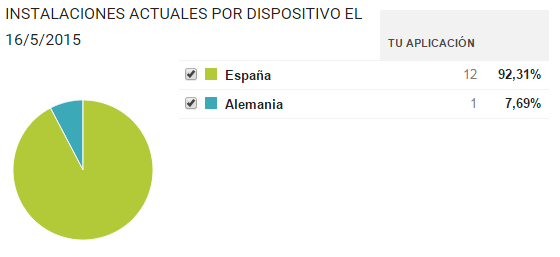
\includegraphics{figs/UsoPorPaises.png}} 
    \caption{Uso por Países de Baldugenda Console Developer} 
    \label{fig:UsoPorPaises} 
  \end{center} 
\end{figure}

Como se puede observar en la figura las instalaciones actuales son 13 y una desde Alemania, que es el Balduser que está de erasmus.

\begin{figure}[H] 
  \begin{center} 
    \scalebox{0.7}{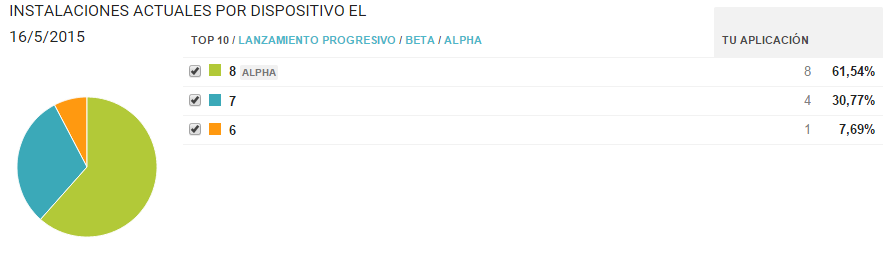
\includegraphics{figs/InstalacionesActuales.png}} 
    \caption{Instalaciones actuales de Baldugenda Console Developer} 
    \label{fig:InstalacionesActuales} 
  \end{center} 
\end{figure}

Las opciones de gráficos facilitan saber cuántos usuarios han actualizado a la versión nueva y cuántos se mantienen en versiones anteriores.
También da la posibilidad de verlo mediante una escala de tiempo


\begin{figure}[H] 
  \begin{center} 
    \scalebox{1}{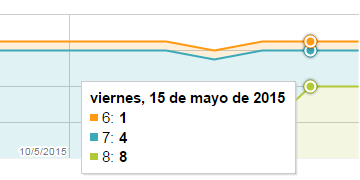
\includegraphics{figs/EscalaTiempo.png}} 
    \caption{Escala de tiempo Console Developer} 
    \label{fig:EscalaTiempo} 
  \end{center} 
\end{figure}

Aparte de todo esto, Google promociona el uso de Google analytics, un servicio web para recopilar datos de interacción del usuario en las aplicaciones que se generen.
En la aplicación de Baldugenda se decidió usar una API de terceros llamada Splunk Mint que se detallara mas adelante para la labor de recopilar información sobre los fallos en la aplicación.
 Al realizar acciones de debugging hay que ponerse en todas las situaciones posibles en las que se pueda llegar a estar en la aplicación, al ser una aplicación móvil no siempre se tendrá la misma cobertura de Internet o las cuentas de Google podrán modificarse.

También puede darse el caso que el móvil falle y se tenga que borrar,  todas estas situaciones hay que tenerlas en cuenta, una de las situaciones que no se suele tener presente cuando no se esta acostumbrado a realizar aplicaciones para móviles es que hay dos posiciones y que dependiendo de que posición se tenga el móvil puede que la información se vea distinta o directamente no se vea.
Puede darse el caso que falle la aplicación en algún punto crítico como puede ser la realización de una escritura en la base de datos o en una llamada al servidor, esas situaciones suelen ser muy comunes al no estar conectado a Internet  todo el rato.

Como al principio no se puede pretender que se sepa en donde va a fallar en cada momento, viene bien instalarse la opción que da Google con su Google analytics o otras opciones de terceros como Splunk mint.
Ya que mientras los usuarios que están haciendo pruebas les falla, se puede configurar para que te llegue al correo el motivo por el que la aplicación ha dejado de funcionar y en que  lineas se ha producido el fallo, gracias a esta información ya se pueden sacar conclusiones de porque ha fallado y como se podría solucionar. Vale de poco pasarse horas y horas probando casos que igual se producen 1 de cada 100.000 veces cuando se ha podido pasar un caso que a una tercera parte de los usuarios les va a suceder.

Los usuarios, la mayoría no sabrán decir lo que les ha pasado cuando ha fallado la aplicación ni tan siquiera lo que estaban haciendo cuando ha dejado de funcionar, por este motivo tener a un chivato que nos diga al menos que botón han pulsado es útil.
 


\subsection{Notificaciones}
\label{subsecc:Notificaciones}

Google proporciona un servicio de notificaciones push muy potente llamado Google Cloud Messaging (GCM), este servicio permite hacer que aparezcan esos mensajes en la pantalla de arriba del móvil cuando llega un mensaje o cuando nos piden vidas en los juegos de las redes sociales.
Gracias a estas notificaciones no se necesita tener la aplicación conectada ya que trabajan sobre un servidor y es el servidor quien se pone en contacto con nosotros.

En el caso de Baldugenda no se han usado este tipo de notificaciones, el uso de notificaciones se ha limitado a las que vienen con los eventos que genera Google Calendar.
Al crear un evento, si el calendario tiene la opción de realizar notificaciones cuando se vaya a producir el evento,   el evento se creara sin ninguna alarma programada pero el propio calendario avisara al usuario con una notificación al móvil o a la versión web si tiene la versión web de Google Calendar abierta.
Para que se produzca la notificación en el móvil el calendario tiene que estar sincronizado con el móvil y actualizado para que se haya cargado los eventos nuevos desde la ultima sincronización, si no se da esa situación la notificación no saltara.
Se decidió no meter alarmas en los exámenes porque eso obligaría al usuario a tener que estar metiéndose en la aplicación cada vez que quisiera desactivar la alarma en cambio al realizarlo mediante Google Calendar y la creacion de eventos, el usuario es libre de realizar las modificaciones en Google Calendar y tener los exámenes en un calendario con las notificaciones activadas.

\subsection{Backup}
\label{subsecc:Backup}

La necesidad del Backup es algo importante en cualquier aplicación en la que el usuario tiene que meter algún dato, a nadie le gusta perder información que ha estado gastando su tiempo escribiendo. Los móviles suelen romperse o estropearse y en esas situaciones perder todo supondría un grave problema, para esas situaciones una copia de seguridad es el mejor salvavidas.
Para el Backup Google tiene opciones tales como las propias implementadas en Android el backup API, que aunque hemos separado las explicaciones en Google y Android, Google compró Android en 2005 y muchas funcionalidades que se pueden encontrar en Android están vinculadas con Google.

Tambien tiene otras opciones más simples como puede ser usar una opción de respaldo en la nube de Google Drive\cite{GDrive}, transparente para el usuario.
La primera opción la ventaja que tiene es que el usuario no tiene que realizar ningún paso para realizar la copia de seguridad, es el propio desarrollador quien prepara todo, pone la clave de la aplicación que se usa en todas los servicios Google para vincular la aplicación con el servicio y después el sistema realiza el backup donde el desarrollador lo escoja. Y Google guarda la información en la nube sin que el usuario pueda acceder a ella, solo se podrá acceder a esa información por medio de la aplicación que ha realizado el backup.

\begin{figure}[H] 
  \begin{center} 
    \scalebox{1}{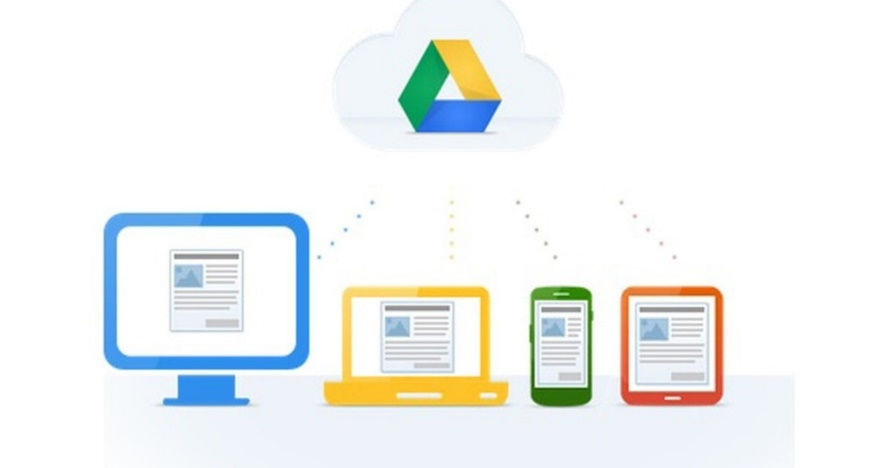
\includegraphics{figs/Drive.png}} 
    \caption{Google Drive Google} 
    \label{fig:Drive} 
  \end{center} 
\end{figure}

La segunda opción parece que tiene más problemas que ventajas pero dependiendo de cómo se use puede ser incluso más útil que la primera.
En esta segunda opción el usuario puede ver en todo momento donde está su información alojada y si no se fía de tenerla en Google Drive puede descargarla y guardarla en su ordenador o mandarla por email.
El problema de tener la copia de seguridad tan accesible es que el usuario puede modificar el fichero, esto podría ser un problema pero con una buena seguridad a la hora de importar la base de datos, esas situaciones no tendrían que repercutir en la aplicación.
Al estar implementando la parte de backup en Drive se encontró que por cada aplicación que se instala los desarrolladores pueden usar una parte del Google Drive si se les da permiso que ni los propios usuarios podrán tocar y sirve como carpeta de preferencias la cual al borrar la aplicación desaparecería.

En Baldugenda esa carpeta no se usó ya que ya se había empezado a usar el sharedpreferences de Android, pero si en alguna aplicación futura se quisiera reducir el espacio que ocupa la aplicación esta carpeta podría resultar de utilidad.
Otra de las ventajas de realizar la copia en Google Drive es que si en un futuro se quisiera compartir información entre usuarios de Baldugenda solo se tendría que modificar la opción de importar y agregar una opción de juntar agenda existente. Con esto se podrían compartir exámenes, asignaturas y el usuario no tendría que estar metiendo las asignaturas ni los exámenes.

El uso de Google Drive es sencillo ya que tiene 3 formas de usarlo y ofrece documentacion para cada una de las formas, mediante REST, mediante la librería java o mediante el sdk de Drive.
El ejemplo que ofrece Google es con el sdk de Drive así que Baldugenda tiene implementada esta opción en el código de Github.
Google Drive ofrece muchas posibilidades a la hora de crear las carpetas y subir los ficheros, se pueden crear ficheros usando tus propias actividades en Android y rellenando todo o puedes usar una actividad que proporciona Google Drive para crear y seleccionar ficheros.

Para el usuario es mucho más cómodo mostrarle algo que le resulte familiar a la hora de hacer elecciones y por eso se optó por usar las actividades que proporciona Google Drive aparte de que tiene un diseño refinado y una cantidad de opciones y posibilidades asombrosas.
Se dieron ciertos problemas a la hora de realizar el backup con Google, ya que al crear carpetas en Drive o ficheros, no se producen inmediatamente y hay situaciones en los que por diversos motivos el servidor está ocupado y tarda un poco más, en esas situaciones el identificador de la carpeta no era accesible desde el momento que se generaba y tardaba un tiempo, esto hacía que fallara seleccionar la carpeta donde el sistema subiria el fichero.
Por ese motivo se decidió separar la parte de la selección de la carpeta de la parte de exportación de la BD.

\subsection{Problemas al desarrollar con Google}
\label{subsecc:Problemas al desarrollar con Google}

La mayoría de los problemas que se encuentran cuando se está trabajando con Google es por el uso de los servicios de Google dentro de la aplicación.
Cuando se intenta implementar algún servicio de Google hay que leerse muy bien el manual del servicio y comprobar que este actualizado. Google tiene un poco desordenado su documentación de los servicios, la ha separado tanto y con tantos enlaces que a veces llega a ser confuso.
Al principio Google explica dentro de su web de APIs que utilidades tienen y como sacarles partido. Para ello separa cada API y hace una especie de guía y después pone un apartado para que se empiece a programar y aquí es donde empieza la confusión, Google suele añadir enlaces a muchos sitios dentro de su documentación para explicar lo más básico del manual, por este motivo hay que tener muy claro donde se tiene que buscar la información.

Una manera de hacer frente a este problema es buscar tutoriales por Internet o video tutoriales donde implementen ese API, y de ahí ya seguir con las funciones propias que tendrá tu aplicación.
El apartado de los credenciales es igual el punto que mayores problemas causan a la hora de hacer que funcione una API al principio, dependiendo qué modo se use, se tiene que activar unas credenciales u otras, aparte cada API necesita un tipo de credencial distinta dependiendo a que recursos quiera acceder la aplicación.
Por ese motivo lo mejor es familiarizarse con la API fuera del proyecto, creando un proyecto pequeño y haciendo que funcione la API por separado y después incluirlo ya funcionando al proyecto que se quiere implementar.
Google dispone de ejemplos en Github de sus APIs, el problema es que esos ejemplos no suelen estar actualizados o no están en todos los modos en los que Google lo ofrece, por ejemplo el API de Google Calendar que se usó en Baldugenda.Google ofrece un acceso a esa API por medio de REST, al ir a buscar ejemplos para esa API se dieron casos de todo tipo, al ser un API que ya tiene distintas versiones, había ejemplos de cada una de ellas pero  de API REST para Android pocos o que no explicaban bien el código. Y en el Github de Google el único ejemplo que había para el API de Google Calendar era haciendo uso de la librería en java.

Aparte del uso de las APIs en Google, otros problemas que han surgido han sido al compartir el enlace de descarga de la aplicación.
La primera opción para compartirlo fue por medio de una comunidad de Google plus,  el fallo que se encontró fue que había algunos Baldusers que no tenían cuenta en Google plus y no querían creársela, así que no podían acceder a la descarga de la aplicación.
Para esos casos se usó los grupos de Google para invitarlos a esos grupos y que pudieran descargarse la aplicación desde ahí.
Algunos Baldusers experimentaron problemas al actualizar baldugenda ya que hay un error en Google play ya reportado por los comunidad de desarrolladores de Google que sucede al corromperse la información de las cuentas vinculadas al dispositivo móvil, por ese motivo Google no permite descargar aplicaciones y exige mucho más espacio del requerido.

Para solucionar el problema se estuvo investigando y la solución era quitar la cuenta de Google del dispositivo y volverla a poner desde cero.
Con eso el Google play cargaría de nuevo la lista de aplicaciones y sus actualizaciones y funcionaria la descarga.
El problema ocasionaba que se les exigía un espacio de memoria altísimo para 2 Mbs que pesaba la aplicación y al no tener espacio suficiente les daba un error al actualizar.


\begin{figure}[H] 
  \begin{center} 
    \scalebox{1}{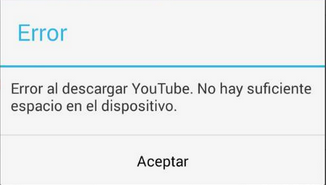
\includegraphics{figs/ErrorGoogle.png}} 
    \caption{Error Google Play} 
    \label{fig:ErrorGoogle} 
  \end{center} 
\end{figure}

Ahora se hablara de problemas más específicos con respecto al calendario y al Drive.

\subsubsection{Problemas Google Calendar}
\label{subsubsecc:Problemas Google Calendar}

Un problema que no se pudo solucionar mediante código fue el problema de la sincronización de Google Calendar con el dispositivo móvil. La idea principal era que cuando se realizaban nuevos eventos en el calendario estos eventos se sincronizaran automaticamente con el calendario del dispositivo, si el Balduser no tenía activada la sincronización por tiempo y la tenía manual no le aparecería en su móvil a menos que le diera a sincronizar.
Para solucionarlo se les comunicó como hacerlo a los Baldusers y los que lo vieron necesario lo usaron.
Otro problema que se encontró al implementar las opciones de calendario fue el uso de la autenticación OAuth2 \cite{Oauth} que requiere el API.
Las explicaciones eran muy confusas a la hora de configurar ya que las ventanas y las opciones que aparecían en la guía de Google eran de versiones anteriores a las configuraciones que tenía que realizar yo.
La forma de solucionarlo fue viendo vídeos donde otros desarrolladores creaban credenciales para APIs de Google que requirieran ese tipo de credenciales y haciendo pruebas se consiguió que empezara a subir la cuota de uso.


\subsubsection{Problemas Google Drive}
\label{subsubsecc:Problemas Google Drive}

Google Drive no dio tantos problemas como en su momento Google Calendar, aun y todo se tuvieron algunos problemas a la hora de implementar la API.
Para facilitar el trabajo con Google Drive y habiendo aprendido de Google Calendar se decidió no perder el tiempo buscando como crear las funciones desde cero y se optó por descargar el ejemplo y coger lo necesario y adaptarlo a Baldugenda.
Cuando se importó el proyecto todo era muy confuso y no se parecía a la forma de trabajar que se había seguido anteriormente en Google Calendar.
Aun y todo se miró el código, se entendió más o menos lo que hacía en cada función,  y se intentó sacar las funciones necesarias al caso de uso de Backup de Baldugenda.
Cuando se sacaron las funciones y se comprobó que funcionaba la selección de ficheros por un lado y la subida de ficheros por otro se intentó juntar.

El problema fue que Google al crear una carpeta mediante el \gls{activity} que dan de ejemplo pasa un tiempo hasta poder usar el identificador de esa carpeta. Y eso producía un fallo en el código ya que al intentar subir a una carpeta que no tenía identificador fallaba el programa.
La solución fue separar por una parte la selección de la carpeta y por otra la subida del fichero, con eso se le daba tiempo a Google a que generara el identificador y de paso el usuario podía comprobar que la carpeta se había seleccionado correctamente.
Antes de optar por esa solución se pensó usar las preferencias de la aplicación para guardar la dirección donde se guardaba la carpeta y de esa manera poder realizar backups periódicos sin depender del usuario, pero el problema seguía siendo el mismo así que se descartó esa opción.

Cuando se implementó el backup no se tuvo en consideración el uso distintos usuarios de Google en el mismo dispositivo. Así que al hacer las pruebas todo iba bien ya que no se modificaba la cuenta, en cambio al usuario sí que se le daba la posibilidad de cambiar las cuentas del Calendar para guardar las cosas. Al ser la forma de conexión distinta no se consiguió usar los certificados creados para el Calendar dentro del Drive.
Se investigó por Internet y en StackOverflow un usuario dio la solución que era agregando el API de Google plus, realizando un borrado del cache de los credenciales y desconectando y volviendo a conectar, ya pedía de nuevo el email de la cuenta a la que se quería acceder.
